% Case-D tangential lever variation for both directions of the achieved initial
% angular offset about t_1. Error bars show the sample standard deviation of the three
% repetitions at each setting.
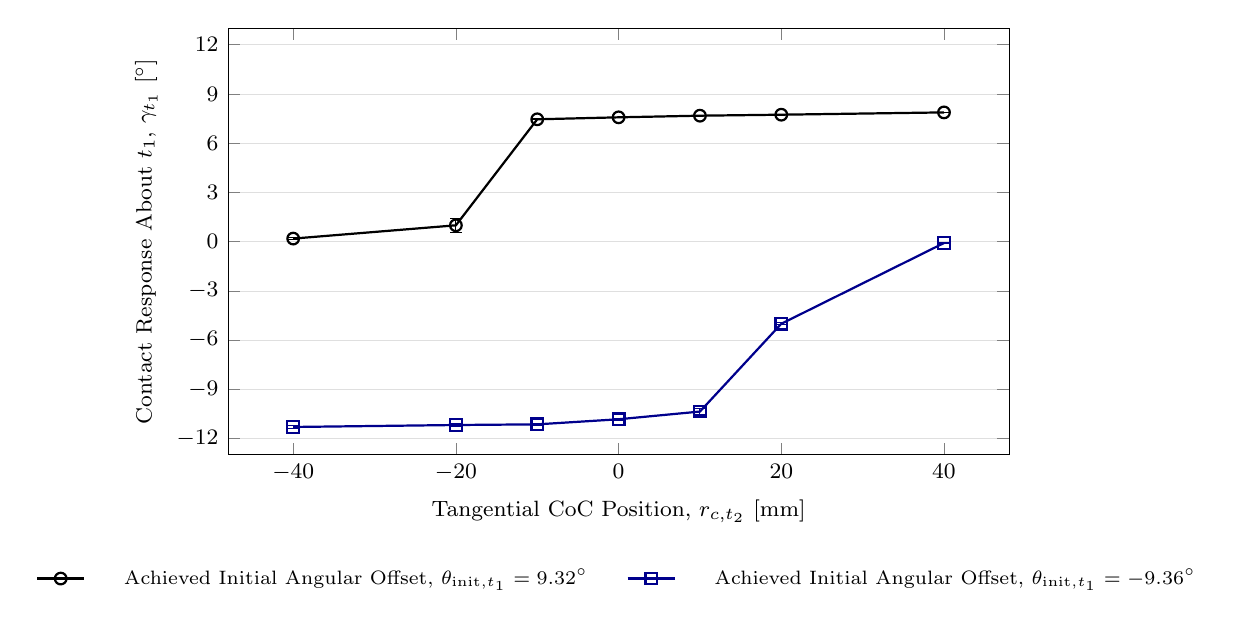
\begin{tikzpicture}
\pgfplotsset{
  every axis/.append style={
    width=11.5cm, height=7.0cm,
    xmin=-48, xmax=48, ymin=-13, ymax=13,
    xtick={-40,-20,0,20,40},
    ytick={-12,-9,-6,-3,0,3,6,9,12},
    ymajorgrids=true,
    xmajorgrids=false,
    grid style={gray!25, very thin},
    tick label style={font=\footnotesize},
    label style={font=\footnotesize},
    legend style={font=\scriptsize, draw=none, fill=none,
                  cells={anchor=west}, at={(0.5,-0.24)}, anchor=north,
                  legend columns=2, column sep=1.2em},
    every axis plot/.append style={thick, mark size=2.1pt},
  },
}
\begin{axis}[
    xlabel={Tangential CoC Position, \(r_{c,t_2}\) [mm]},
    ylabel={Contact Response About \(t_1\), \(\gamma_{t_1}\) [\(^\circ\)]},
  ]
\addplot[black, mark=o, error bars/.cd, y dir=both, y explicit] coordinates {
  (-40,0.18) +- (0,0.07) (-20,0.99) +- (0,0.44)
  (-10,7.45) +- (0,0.02) (0,7.57) +- (0,0.01)
  (10,7.67) +- (0,0.01) (20,7.73) +- (0,0.01)
  (40,7.87) +- (0,0.01)};
\addlegendentry{Achieved Initial Angular Offset, \(\theta_{\mathrm{init},t_1}=9.32^\circ\)}
\addplot[blue!55!black, mark=square, error bars/.cd, y dir=both, y explicit] coordinates {
  (-40,-11.30) +- (0,0.11) (-20,-11.18) +- (0,0.09)
  (-10,-11.14) +- (0,0.07) (0,-10.83) +- (0,0.06)
  (10,-10.36) +- (0,0.21) (20,-5.01) +- (0,0.07)
  (40,-0.09) +- (0,0.01)};
\addlegendentry{Achieved Initial Angular Offset, \(\theta_{\mathrm{init},t_1}=-9.36^\circ\)}

\end{axis}
\end{tikzpicture}
